\section{Running the benchmarks}

After developing all the flags that control the behavior of the compiler with
regards to undefined behavior exploitation, we started the performance
experiments. There is a total of 20 configurations that we used:
\begin{itemize}
  \item baseline, i.e. without any undefined behavior flag
  \item one undefined behavior flag at a time
  \item all undefined behavior flags combined
\end{itemize}

Considering that we have 25 benchmarks, each with a variable number of tests
that can finish in a matter of minutes or in a matter of hours, the whole
benchmarking process took us approximately two weeks for each of our servers,
i.e. an Intel Xeon E5-2680 v2 @ 3.60GHz and an arm Neoverse-N1 @ 3.00 GHz.

Before analyzing the results we had to make sure that the benchmarking
environment is stable so that our results do not show a high degree of variance.
In the past semester we ran a couple of experiments on the Intel server and we
have seen a satisfactory level of variance, e.g. 2\%. However, this semester we
also acquired an arm server on which we ran the experiments and which showed
levels of variance way above the satisfactory threshold. This was a major
problem as no significant conclusion could be drawn from benchmarks with this
level of instability.

Figure~\ref{fig:EncoderModeSpeed6TwoPassInputBosphorus4K} shows a case of
variance in the aom-av1 benchmark. While configurations such as
-fconstrain-shift-value, -fdrop-align-attr, -fdrop-deref-attr have an
insignificant variance, configurations such as "-fdrop inbounds-from-gep -mllvm
-disable-oob-analysis" or -fignore-pure-const-attrs show variances between the
min value and the max value of 62\% or 106\%.

To solve the variance issues we found the following two methods to be effective:
\begin{itemize}
  \item Use numactl to pin the benchmarking process to a specific NUMA node
  \item Reduce the processor frequency
\end{itemize}

Figure~\ref{fig:EncoderModeSpeed11RealtimeInputBosphorus4K} shows the advantages
of these two techniques on the baseline configuration. Running at 3.00GHz
without numactl exposes outliers that are not found in the versions with reduced
frequency and numactl enabled. Even though for this specific case the variance
at 1.50GHz and at 2.00GHz seems acceptable, there are other tests in aom-av1
that do not show satisfactory variance for 1.50GHz and 2.00GHz. Because of this
we chose to decrease the frequency to 1.00GHz.

The question on why the benchmarks are more unstable on arm than on x86 still
persists. We have a couple of theories on why this might happen but we need to
do more experiments in order to validate them. They include: CPU frequency
instability caused by the thermal controllers or unstable memory access times
caused by the memory access patterns displayed by the benchmarks. 

\begin{figure}[H]
  \centering
  \includesvg{EncoderModeSpeed11RealtimeInputBosphorus4K}
  \caption{Improvement of stability using numactl and frequency dropping}
  \label{fig:EncoderModeSpeed11RealtimeInputBosphorus4K}
\end{figure}

After solving the instability problems, we continued to gather and analyse the
results on both Intel and arm.

On one hand, Figure~\ref{fig:x86_affected_bms_per_flag} and
Figure~\ref{fig:arm_affected_bms_per_flag} present the quantitative impact of
each flag over the benchmark suite, i.e. how each flag affects the benchmarks.
We define affected benchmarks as benchmarks for which there exists a performance
improvement over 2\% or a performance decrease over 2\%.

In these figures we expand the definition of a benchmark. In the beginning of
this section we stated that our suite consists of 25 benchmarks. However, these
25 benchmarks can be considered as 25 separate application that, in turn,
contain a variable number of sub-benchmarks, or tests. This expansion results in
over 140 benchmarks.

We expected the flags to affect differently the benchmarks on the two hardware
architectures since they use different operating system configurations and have
different hardware characteristics. The cumulative effect of the flags in bigger
on arm than on x86. Plus, for each individual flag, arm has a bigger impact on
the benchmark than x86. We plan to answer in the following semester what is the
exact cause of these differences.

\begin{figure}[H]
  \centering
  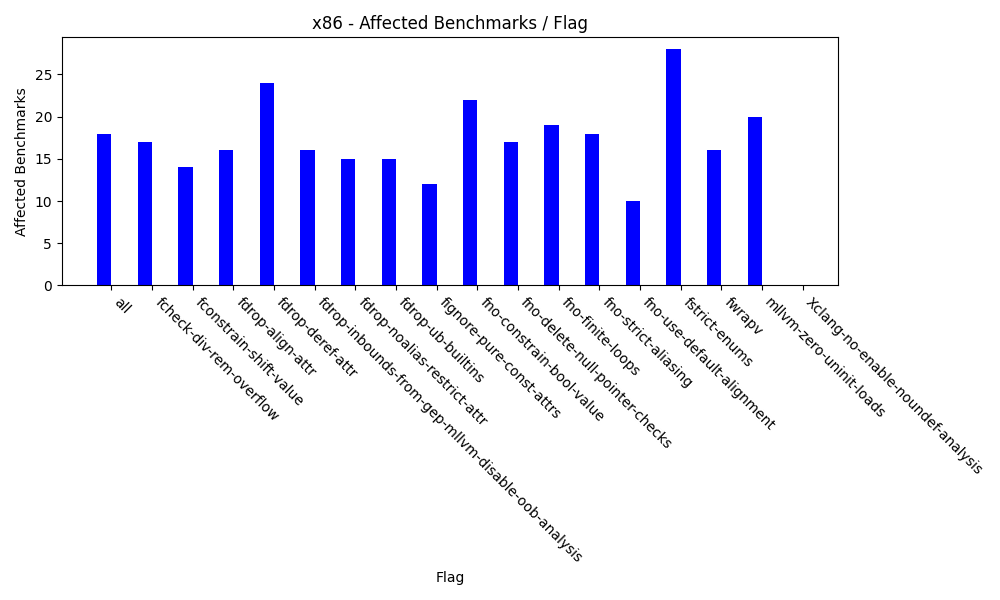
\includegraphics[scale=0.6]{x86_affected_bms_per_flag}
  \caption{Number of affected benchmarks by each flag on x86 for -O2}
  \label{fig:x86_affected_bms_per_flag}
\end{figure}

\begin{figure}[H]
  \centering
  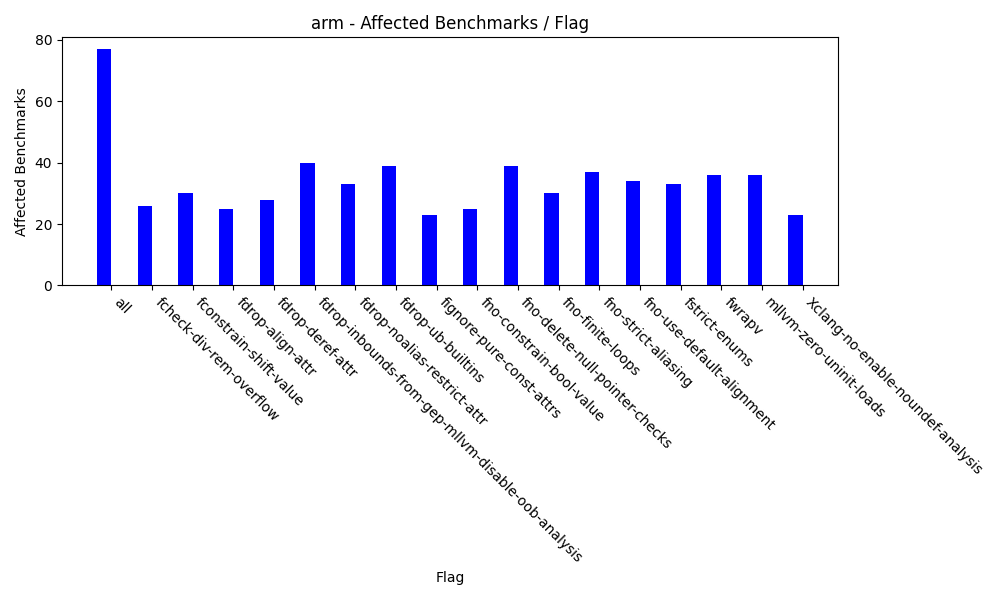
\includegraphics[scale=0.6]{arm_affected_bms_per_flag}
  \caption{Number of affected benchmarks by each flag on arm of -O2}
  \label{fig:arm_affected_bms_per_flag}
\end{figure}

On the other hand, Figure~\ref{fig:x86_impact_per_flag} and
Figure~\ref{fig:arm_impact_per_flag} present the qualitative impact of each flag
over the benchmark suite. No flag exhibits overall negative impact or overall
positive impact. Each benchmark is affected differently by the same flag. This
happens because each benchmarked application contains different resource
utilization patterns.

\begin{figure}[H]
  \centering
  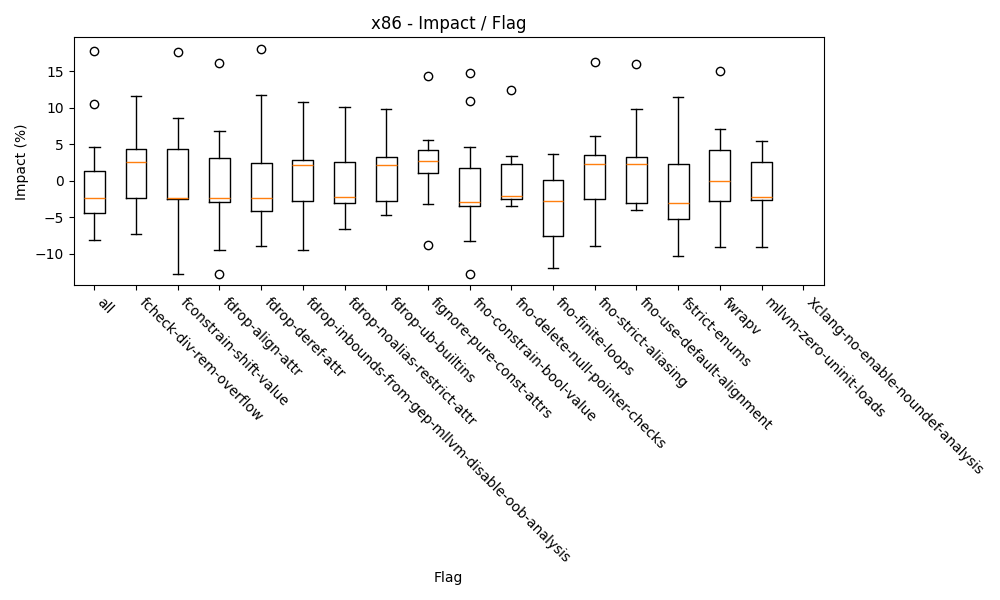
\includegraphics[scale=0.6]{x86_impact_per_flag}
  \caption{Impact of each flag on the suite on x86 for -O2}
  \label{fig:x86_impact_per_flag}
\end{figure}

\begin{figure}[H]
  \centering
  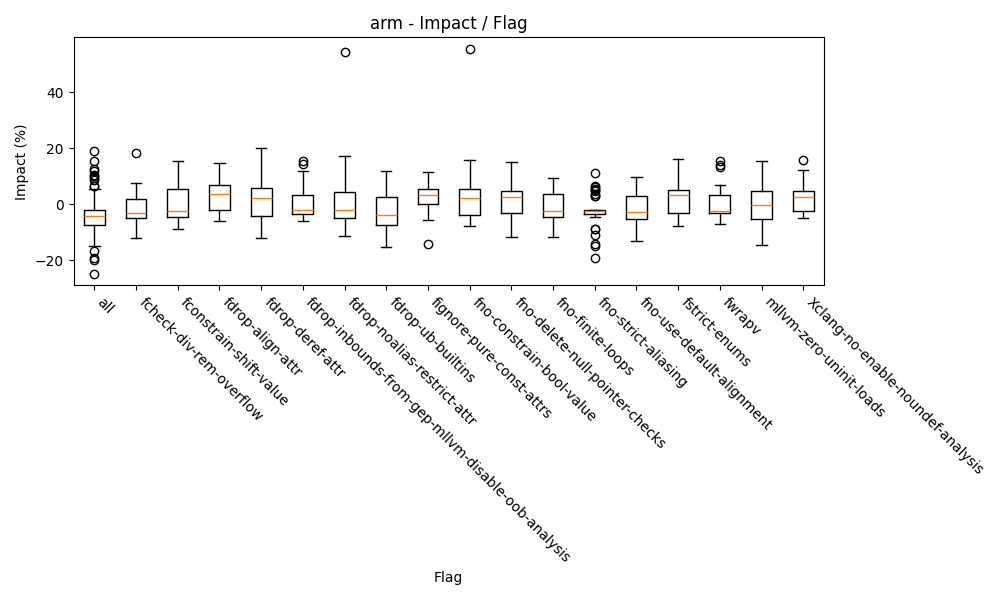
\includegraphics[scale=0.6]{arm_impact_per_flag}
  \caption{Impact of each flag on the suite on arm for -O2}
  \label{fig:arm_impact_per_flag}
\end{figure}

Currently we have the -O2 numbers for both Intel and arm, we plan to continue to
gather the numbers for -O3, -Os and -Oz.

While we are gathering the numbers for the rest of optimization levels, we
started the analysis of the performance regressions for -O2 on x86. The next
section talk about the analysis process and current findings.
